\section{Implementation}
\label{sec:implementation}

We implement \system as a header-only C++17/CUDA library with 7,574 lines in public and internal headers.  CMake selects CUDA architecture 7.5 by default, and preliminary measurements use release builds.  Access traits abstract graph storage, compile-time policies define algorithm behavior, and runtime descriptors provide query sources and parameters.

\paragraph{Graph and query state.}
The source-oriented strategy reads outgoing CSR.  The destination-oriented strategy also reads incoming CSR.  Weighted algorithms use an aligned edge-weight array.  One engine workspace owns the vertex-major value matrix; current, next, and cumulative query masks; compact union frontiers; scan offsets; access counters; and the active-query set.  When $N>Q$, batches reuse this workspace, so memory scales with resident queries rather than window size.

For a $w$-byte value, the value matrix requires $w|V|Q$ bytes.  Three 64-bit masks add $24|V|$ bytes, independent of $Q$ up to 64.  Compact lists, flags, and scan offsets add $O(|V|)$ storage.  Table~\ref{tab:workspace} summarizes the principal structures; graph CSR and its transpose are reported separately in the evaluation.

\begin{table}[t]
  \centering
  \caption{Principal device structures, excluding graph CSR and its transpose.}
  \label{tab:workspace}
  \small
  \begin{tabular}{lll}
    \toprule
    Structure & Approx. bytes & Lifetime \\
    \midrule
    typed values & $w|V|Q$ & batch \\
    three query masks & $24|V|$ & batch \\
    union vertex lists & $2s_v|V|$ & batch \\
    scan/flag arrays & $O(|V|)$ & batch \\
    phase distances & $2L|V|$ & graph reuse \\
    counters/active word & $O(1)$ & iteration \\
    \bottomrule
  \end{tabular}
\end{table}

\paragraph{GPU mapping.}
This paragraph contains the hardware-specific mapping deliberately omitted from the conceptual design.  \sharedexpand assigns one active union vertex to a cooperative execution group; the current default uses a warp for a vertex and distributes high- and low-degree rows across blocks for load balance.  \coalescedgather maps the query identifier to the contiguous dimension of a CUDA block while holding a destination row fixed.  As Figure~\ref{fig:layout} shows, this mapping follows the vertex-major state layout and turns one vertex's query values into consecutive accesses.

\begin{figure}[t]
  \centering
  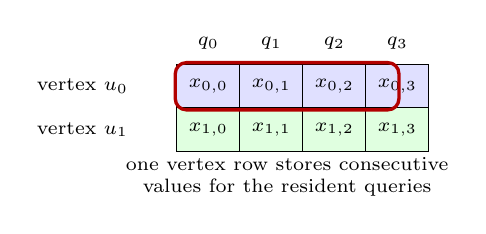
\begin{tikzpicture}[
      font=\scriptsize,
      cell/.style={draw, minimum width=8mm, minimum height=5.5mm, inner sep=0pt},
      lab/.style={align=right}
    ]
    \node[lab] at (-1.2,0) {vertex $u_0$};
    \node[lab] at (-1.2,-0.55) {vertex $u_1$};
    \foreach \x/\q in {0/0,1/1,2/2,3/3} {
      \node at (0.4+0.8*\x,0.55) {$q_{\q}$};
      \node[cell, fill=blue!12] at (0.4+0.8*\x,0) {$x_{0,\q}$};
      \node[cell, fill=green!12] at (0.4+0.8*\x,-0.55) {$x_{1,\q}$};
    }
    \draw[very thick, red!70!black, rounded corners] (-0.02,-0.3) rectangle (2.82,0.3);
    \node[align=center] at (1.4,-1.15) {one vertex row stores consecutive\\values for the resident queries};
  \end{tikzpicture}
  \caption{Vertex-major $V\!\times\!Q$ state layout used by \coalescedgather.  Holding the graph vertex fixed while varying the query identifier turns the query dimension into a contiguous access sequence.}
  \Description{A two-row value matrix with vertices as rows and resident queries as contiguous columns. A highlighted row contains all query values for one graph vertex.}
  \label{fig:layout}
\end{figure}


\paragraph{Frontier construction.}
Atomic updates merge successful query bits at a destination.  A first-writer test records whether the destination needs a compact-list entry; a prefix scan then produces the next union frontier and counts unique vertices and query--edge pairs.  Both traversal strategies emit the same compact format.  These operations are included in end-to-end time because omitting them would overstate the benefit of sharing.

\paragraph{Execution variants.}
The implementation retains vertex-parallel, query-parallel, and shared-vertex expansion kernels for controlled comparison.  The aligned path has a direct row--query kernel and a neighbor-tiled shared-memory variant.  The direct kernel uses 128 CUDA threads: it processes two destination rows at $Q=64$ and four at $Q=32$.  Current focused experiments find that synchronization and shared-memory traffic outweigh neighbor-identifier reuse in the tiled variant, so the direct path is the default.  These variants are implementation alternatives, not separate paper contributions.

\paragraph{Scheduled activation.}
Per-query start levels are stored in a host-generated schedule and converted to an activation mask at each global step.  Activating a query initializes only its source value and source frontier bit.  Inactive queries are filtered in both strategies, so offsets require neither clearing nor reallocating the $V\!\times\!Q$ matrix.

\paragraph{Strategy selection.}
Before a hybrid decision, a GPU kernel sums union edges, query-weighted edges, and active pairs into 64-bit counters.  The current engine copies them to the host before launching the selected strategy.  This path is useful for instrumentation but introduces per-iteration synchronization.  The final implementation should compare host selection with a device-side decision or a CUDA Graph path; all end-to-end measurements include the current control cost.

\paragraph{Phase-index persistence.}
The reusable index stores graph dimensions, landmark identifiers and weights, and landmark-major 16-bit distances.  Build and load are separate code paths.  The online runner loads an existing index when available and charges query-dependent evaluation to the window, while reporting build time, load time, size, and break-even windows separately.

\paragraph{Measurement and correctness.}
The runner executes input-order, batch-only, offset-only, and full schedules through the same engine.  It reports GPU execution time, scheduling time, union and query-weighted edge counts, and result fingerprints.  Focused profiling uses NVIDIA Nsight Compute; complete runs use CUDA events and host timers.  Debug tests compare all output values, while experiment runs additionally store per-query fingerprints.  The runtime rejects batches above 64 queries, invalid sources, unsupported schedules, and aligned aggregation without incoming adjacency.

\paragraph{Current engineering boundary.}
The prototype contains exact query masks, typed BFS/SSSP/widest-path policies, both traversal strategies, the phase index, grouping and offset search, and the threshold selector.  It does not yet contain the calibrated model in Section~\ref{sec:selector}.  A final claim about adaptive strategy selection is contingent on implementing and evaluating that model.
